\subsection{测度支集的刻画}

按定义，若函数 \(f \in \mathcal{K}(\mathrm{X};\mathbf{C})\) 的支集与测度 \(\mu\) 的支集不相交，则 \(\mu(f) = 0\) ；但下述更精确的结果成立：

命题 8. --- 设 \(\mu\) 是局部紧空间 \(X\) 上的一个测度。对每个函数 \(f \in \mathcal{K}(X; \mathbf{C})\) （在 \(\operatorname{Supp}(\mu)\) 上为零），有 \(\mu(f) = 0\) 。

设 \(\mathrm{K} = \operatorname{Supp}(f)\) ， \(\mathrm{S} = \operatorname{Supp}(\mu)\) 。给定一个数 \(\varepsilon > 0\) ，设 \(\mathrm{V}\) 是 \(x \in \mathrm{X}\) （\(|f(x)| < \varepsilon\) ）所成之集；按假设 \(\mathrm{V}\) 是包含 \(\mathrm{S}\) 的开集，因此 \(\complement \mathrm{S}\) 是紧集 \(\complement \mathrm{V}\) 的一个邻域。由此可知，存在一个连续映射 \(h\) ，它把 \(\mathrm{X}\) 映到 {[}0,1{]} 中，在 \(\complement \mathrm{V}\) 上等于 1 且支集含于 \(\complement \mathrm{S}\) （§1, No.~2, 引理 1）。由于 \(fh\) 的支集与 \(\mathrm{S}\) 不相交，故 \(\mu(fh) = 0\) 。另一方面， \(f = fh\) 在 \(\mathrm{K} \cap \complement \mathrm{V}\) 上成立，且 \(|fh| \leqslant |f|\) 在 \(\mathrm{X}\) 上成立，故 \(|f - fh| \leqslant 2\varepsilon\) 在 \(\mathrm{X}\) 上成立（由 \(\mathrm{V}\) 的取法）。最后注意，存在一个数 \(\mathrm{M}_{\mathrm{K}}\) ，使得 \(|\mu(g)| \leqslant \mathrm{M}_{\mathrm{K}} \| g\|\) 对每个函数 \(g \in \mathcal{K}(\mathrm{X};\mathbf{C})\) （支集含于 \(\mathrm{K}\) ）成立；由于 \(f - fh\) 的支集含于 \(\mathrm{K}\) ，故 \(|\mu(f - fh)| \leqslant 2\mathrm{M}_{\mathrm{K}}\varepsilon\) ，从而 \(|\mu(f)| = |\mu(f - fh)| \leqslant 2\mathrm{M}_{\mathrm{K}}\varepsilon\) ；由于 \(\varepsilon\) 是任意的，故 \(\mu(f) = 0\) 。

推论 1. --- 若两个函数 \(f, g\) （在 \(\mathcal{K}(\mathrm{X};\mathbf{C})\) 中）在 \(\operatorname{Supp}(\mu)\) 上相等，则 \(\mu(f) = \mu(g)\) 。

推论 2. --- 设 \(\mu\) 是 X 上的一个正测度；若 \(f \in \mathcal{K}(X; \mathbf{C})\) 使 \(f(x) \geqslant 0\) 在 \(\operatorname{Supp}(\mu)\) 上成立，则 \(\mu(f) \geqslant 0\) 。

因为 \(f = |f|\) 在 \(\operatorname{Supp}(\mu)\) 上成立，故由推论 1 得 \(\mu(f) = \mu(|f|) \geqslant 0\) 。

推论 3. --- 设 \(\mu\) 是 X 上的一个有界测度；若 \(f \in \mathcal{K}(X; \mathbf{C})\) 使 \(|f(x)| \leqslant a\) 在 \(\operatorname{Supp}(\mu)\) 上成立，则 \(|\mu(f)| \leqslant a \| \mu \|\) 。

因为 \(\operatorname{Supp}(|\mu|) = \operatorname{Supp}(\mu)\) ，并且若 \(h\) 是 X 到 \([0,1]\) 中的一个连续映射，在 \(\operatorname{Supp}(f)\) 上等于 1 且具紧支集，则 \(|f(x)| \leqslant ah(x)\) 在 \(\operatorname{Supp}(\mu)\) 上成立，因此

\[
| \mu | (| f |) \leqslant a | \mu | (h) \leqslant a \| \mu \|
\]

这是依据推论 2；于是结论由 §1, No.~6 的公式 (13) 得出。

命题 9. --- 设 \(\mu\) 是 X 上的一个正测度；若 \(f\) 是 \(\mathcal{K}_{+}(X)\) 中满足 \(\mu(f)=0\) 的函数，则 \(f\) 在 \(\operatorname{Supp}(\mu)\) 上为零。

设 \(x\) 是 \(X\) 中满足 \(f(x) > 0\) 的一点；我们证明 \(x\) 不属于 \(\operatorname{Supp}(\mu)\) 。因为存在一个紧邻域 \(V\) （\(x\) 的）及一个数 \(a > 0\) ，使得 \(f(y) \geqslant a\) 在 \(V\) 上成立。若 \(g\) 是任一 \(\geqslant 0\) 且支集含于 \(V\) 的连续函数，我们证明 \(\mu(g) = 0\) ；事实上，若令 \(b = \|g\|\) ，则 \(g \leqslant bf/a\) ，于是 \(\mu(g) \leqslant b\mu(f)/a = 0\) 。

命题 10. --- 设 \(\mu\) 是局部紧空间 \(X\) 上的一个测度；对每个函数 \(g \in \mathcal{C}(X; \mathbf{C})\) ，测度 \(g \cdot \mu\) 的支集是 \(T\) ，即点 \(x \in \operatorname{Supp}(\mu)\) （\(g(x) \neq 0\) ）所成之集的闭包。

设 \(S = \operatorname{Supp}(\mu)\) ；设 \(x_{0}\) 是不属于 T 的一点；存在 \(x_{0}\) 的一个开邻域 V，使在 \(V \cap S\) 的每一点处 g 为零；若 \(f \in \mathcal{K}(X; \mathbf{C})\) 的支集含于 V，则 fg 在 S 上为零，因此（命题 8） \(\mu(gf) = 0\) ；换言之， \(g \cdot \mu\) 在 V 上的限制为零。

反之，设 \(g \cdot \mu\) 在某点 \(x_{0} \in X\) 的一个开邻域 W 上的限制为零，我们证明不存在 \(W \cap S\) 中使 g \(\neq 0\) 的点。事实上，倘若存在这样一点 y，则存在包含于 W 的 y 的一个紧邻域 U，在其每一点 x 处 \(g(x) \neq 0\) ；于是每个支集含于 U 的函数 \(f \in \mathcal{K}(X; \mathbf{C})\) 都可写成 f = gh，其中 \(h \in \mathcal{K}(X; \mathbf{C})\) 的支集含于 \(U \subset W\) ；由此将得 \(\mu(f) = \mu(gh) = 0\) ，与假设 \(y \in S\) 相矛盾。

\pandocbounded{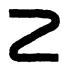
\includegraphics[keepaspectratio]{images/part001_a1e78629.jpg}}

注意，T 含于 \(\mu\) 的支集 S 与 g 的支集之交，但未必等于这一交。例如，若 X = R， \(\mu\) 是点 0 处的 Dirac 测度，且 \(g(x) = x\) ，则 \(g \cdot \mu = 0\) ，尽管 g 与 \(\mu\) 的支集之交退缩为点 0，因而是非空的。

推论. --- 为使测度 \(g \cdot \mu\) 为零，必须且只须 g 在 \(\mu\) 的支集上为零。

命题 11. --- 每个具紧支集的测度都是有界的。

因为 \(|\mu|\) 也是具紧支集的测度，故可只限于 \(\mu \geqslant 0\) 的情形；若 \(h\) 是 \(X\) 到 {[}0,1{]} 中的一个连续映射，具紧支集且在 \(\operatorname{Supp}(\mu)\) 上等于 1，则对每个函数 \(f \in \mathcal{K}(X; \mathbf{C})\) ，有 \(|f(x)| \leqslant \|f\|h(x)\) 在 \(\operatorname{Supp}(\mu)\) 上，因此（命题 8 的推论 2） \(\mu(|f|) \leqslant \mu(h)\|f\|\) ，这就证明了该命题（§1, No.~8）。

